\chapter{Literature Review}
\label{chap:lit-review}

\section{Introduction}

\section{Quadcopters}

\subsection{Modelling}

When designing a control system, arguably the most crucial part of the process is to derive an accurate mathematical model of the plant that is to be controlled. The plant in this case is a unmanned aerial vehicle (UAV) in a `quadcopter' configuration. 

As part of the X-4 Flyer project,~\cite{hamel2002dynamic} set out to derive a simple model for their plant using only rigid body dynamics and abstract force and torque actuators. As stated by~\cite{Pounds2010c}, this model, like many others that were derived at the time, represents the quadcopter as a rigid body mass with inertia and autogyroscopics, affected only by gravity and actuator torques.~\citeauthor{Pounds2010c} further argues that these simple quadcopter models do not accurately represent the complex helicopter-like behaviour exhibited by real quadcopters at high rotor speeds. These high-speed rotor effects include the blade flapping effect, which affect the quadcopter frame's oscillatory modes, rotor flapping from varying quadcopter yaw angles, and variable airflow velocities over the rotor blades from varying roll and pitch angles.

In an attempt to create a quadcopter model that will allow a quadcopter to be more accurately controlled at high rotor speeds,~\citeauthor{Pounds2010c} set out to derive a model incorporating the rigid body dynamics, as well as the aerodynamic effects mentioned earlier. Their model is based on the diagram given in Figure~\ref{fig:chap2-quad-model}.

\begin{figure}
  \centering
  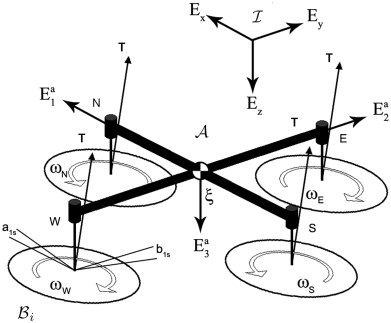
\includegraphics[width=0.5\textwidth]{figures/chapter2/pounds_quad-model.jpg}
  \caption[A diagram of the quadcopter model, including the blade flapping dynamics.]{A diagram of the quadcopter model, including the blade flapping dynamics. Adapted from~\cite{Pounds2010c}.}
\label{fig:chap2-quad-model}
\end{figure}

Their resulting model was used to develop a simple hovering Proportional Integral Differential (PID) attitude and altitude controller for the purpose of model verification. The results show that the drone stabilised itself in indoor flight with $\pm1$\textdegree of precision and $\pm5$\textdegree of precision during outdoor flight. The lower precision during outdoor flights is due to the added wind disturbances, etc. Thus, the model, as it stands, is sufficiently accurate to safely control a drone for hovering. However, they did not compare their model, which includes aerodynamic effects, against the model of~\citeauthor{hamel2002dynamic}, which is based on rigid body dynamics. 

\subsection{Control}

\subsubsection{Introduction}

After an accurate model, the next most important part of a good control system is the controller itself. Many controllers have been implemented and tested on quadcopters over the years. Different control strategies have also been investigated. Some of the most prevalent control strategies and controllers are discusses.

\subsubsection{Indoor vs. Outdoor Control}

There are different types of quadcopters, each of them equipped with different sensors and equipment. The two main types of quadcopters are indoor and outdoor quadcopters. Each of them work in different ways and implement very different control schemes. 

Indoor drones may or may not come equipped with an on-board inertial measurement unit (IMU), which includes an accelerometer and gyroscope, for stability control. However, they commonly rely soley an external motion detection system which tracks the drones movements, providing position and rotation (also known as pose) feedback to controller, thereby closing the control loop. These drones are exceptionally accurate and capable of performing remarkable acrobatic feats. However, they are restricted to carefully controlled indoor environments.

Outdoor drones, without the luxury of having very accurate external sensors available, have to rely on their on-board sensors to provide the controller with pose feedback. These on-board sensors these drones come equipped with may vary between quadcopter platforms, however they almost certainly come equipped with an IMU to provide pose data. However, since the IMU readings for position data drifts with time due to integration errors, a global positioning system (GPS) sensor is added to provide a base-line reading for a quadcopter's position. Other sensors that may be included are magnetometers, barometers, visual feedback sensors and sonar sensors. To combine the readings of the different sensors, a filtering technique, such as the Extended Kalmann Filter, is used. The pose error of the combination of the different readings are, in theory, less than the most accurate sensor in the suite, but this has not yet been proven. 

\subsubsection{Hovering Control}

Stable hovering of a quadcopter has been the focus of many projects and research papers in the past 15 years. As a result, many different control methods and schemes have been investigated, implemented and compared. Hovering control refers to a quadcopters ability to hover and remain stable at a set point in 3-dimensional space.

\cite{bouabdallah2004pid}, as part of their `OS4' project, compared the modern linear quadratic regulator (LQR) and classic PID controller with one another, with respect to the control performance (disturbance rejection, reference tracking, etc.), of a quadcopter.

They found that the PID controller produced better results than the LQR in terms of reference tracking and dynamic performance. This was a surprising result, since LQR controllers normally excel at controlling unstable, underactuated plants such as a quadcopter platform. They suspect that the reason for this result may be because they neglected the effects of actuator dynamics, such as blade and rotor flapping, in their drone model. However, they do expect that an LQR controller will produce superior results if these effects are taken into account. 

Some researchers have also investigated controlling a drone using an H-infinity (H$_{\inf}$) control structure and a model predictive controller (MPC).

Most notably,~\cite{raffo2010integral} have done extensive research on this topic. MPC's are computationally efficient and modern controllers that drive a plant's state to a reference state within predefined constraints (eg.\ motor saturation, model dynamics, etc.), while a properly designed non-linear H$_{\inf}$ controller is very good at rejecting disturbances (eg.\ wind gusts, motor vibrations, etc.) and are robust to model uncertainties. They opted to combine the two controllers in an intelligent manner in order to extract the most efficient performance out of their drone. 

In their simulations they found that the resulting controller performed admirably, presenting good reference tracking, proving to be robust with uncertain mass and inertia terms and deals well with disturbances on all 6 degrees of freedom at different points in time. However, they are yet to implement and test their controller configuration on a real drone. Although the algorithms and methods they used are computationally efficient, it may still prove to be too computationally intensive for the limited computing power on-board a drone. Given the fast growth of processing power, however, this controller configuration may become a more viable option in the near future. 

Controllers for enabling a drone to hover have already been successfully designed and implemented, and it is therefore possible to accurately control a drone during hovering operations. 

\section{Computer Vision}

\subsection{Introduction}

Computer vision is a diverse field which primarily focuses on devising methods for acquiring, processing, analysing and understanding images captured of the real world. There are various sub-fields of research, but a common theme across all the fields is to mimic the human ability to perceive and understand an image, and perhaps react accordingly to different visual inputs. 

The fields of interest for this thesis, is the object detection, tracking and pose estimation fields. This section aims to discuss the work that has been done in these fields. 

\subsection{Camera Matrix}

An image is a collection of 2-dimensional vectors representing a collection of 3-dimensional space vectors. These collections of vectors are related by a matrix $C$, known as the camera matrix. The camera matrix contains the intrinsic parameters of the camera that recorded the image, i.e.\ the focal lengths and principle point of the image, as well as the extrinsic parameters of the camera, i.e.\ the translation and rotation information. The camera matrix $C$ given is given by Equation~\ref{eq:chap2-cam-matrix}, as derived by~\cite{heikkila1997four}. 

\begin{equation}
  \label{eq:chap2-cam-matrix}
  C = 
  NP
\end{equation}

where $N$ is given by the matrix in Equation~\ref{eq:chap2-cam-intrinsic}.

\begin{equation}
  \label{eq:chap2-cam-intrinsic}
  N = 
  \begin{bmatrix}
    f_x & 0   & u_0 \\
    0   & f_y & v_0 \\
    0   & 0   & 1   \\
  \end{bmatrix}
\end{equation}

Here, $f_x$ and $f_y$ describe the focal lengths of the camera and $u_0$ and $v_0$ are the principal points. 

The pose matrix $P$ is given by the matrix in Equation~\ref{eq:chap2-cam-extrinsic}.

\begin{equation}
  \label{eq:chap2-cam-extrinsic}
  P = 
  \begin{bmatrix}
    R | T
  \end{bmatrix}
  =
  \begin{bmatrix}
    r_{11} & r_{21} & r_{31} & t_1 \\
    r_{21} & r_{22} & r_{32} & t_2 \\
    r_{31} & r_{23} & r_{33} & t_3 \\
  \end{bmatrix}
\end{equation}

In the matrix $P$, $R$ is a $3\times3$ matrix describing the rotation of the camera, and $T$ is a three-dimensional vector describing the translation of the camera. 


If the camera matrix $C$ is known, the 3-dimensional coordinates for any 2-dimensional image can be determined by the relation given in Equation~\ref{eq:chap2-2d-to-3d}. The camera matrix is commonly determined through some camera calibration procedure. One such a procedure is discussed in Section~\ref{sec:chap2-cam-calibration}.

\begin{equation}
   \label{eq:chap2-2d-to-3d}
   \begin{bmatrix}
     x_c & y_c & 1 \\
   \end{bmatrix}^T
   = C
   \begin{bmatrix}
     x_w & y_w & z_w & 1 \\
   \end{bmatrix}^T
 \end{equation}

\subsection{Camera Calibration}
\label{sec:chap2-cam-calibration}

A properly calibrated camera is a very important part of any computer vision system, since the accuracy of the data extracted from an image may strongly depend on the accuracy of the calibration. The goal of a camera calibration procedure is to produce the complete camera matrix $C$, as given in Equation~\ref{eq:chap2-cam-matrix}, as well as finding the camera's distortion coefficients introduced by low-quality or fish-eye lenses. There are various camera calibration procedures available, from the two-step calibration described by~\cite{melen1994geometrical} to the classical approach given by~\cite{slama1980manual}, where a non-linear error function is minimised. However, the minimisation problem presented by~\citeauthor{slama1980manual} is computationally inefficient and slow, while~\citeauthor{melen1994geometrical}'s method does not account for image distortion and correction. A popular calibration method is the four-step method, proposed by~\cite{heikkila1997four} as an extension to the two-step method which was the prevalent at the time.

The `calibrateCamera()' function of the OpenCV computer vision library [\cite{bradski2000opencv}], makes use of the four-step method. The fine details of the method is beyond the scope of this research, however a broad overview of the steps and equipment required to calibrate a camera, is provided. 

To perform the calibration and find the camera matrix, OpenCV requires two sets of data: one two-dimensional image data set, $[x_c\;y_c\;1]$, as well as a set of corresponding three-dimensional data points, $[x_w\;y_w\;z_w\;1]$. This implies that image data of an object where the dimensions and coordinates of certain features are known, must recorded. In practice, any well-characterised object can be used for calibration. For example, some calibration methods rely on a three-dimensional cube covered in precisely laid out markers. However, since manufacturing and distributing such precisely constructed objects to a large audience is infeasible, and therefore OpenCV opts to use the more convenient flat, regular pattern, such as chessboard or asymmetrical dot pattern. Figure~\ref{fig:chap2-calib-pattern} shows an example of a typical chessboard pattern generated by OpenCV.\@ With these flat patterns, the features used to populate the data sets would be the square corners on a chessboard, i.e.\ where a black block meets another black block, or the dots on an asymmetric dot pattern. The drawback to this approach, however, is that multiple views of the flat calibration pattern is required, whereas a single image of the three-dimensional object would suffice. 

\begin{figure}
  \centering
  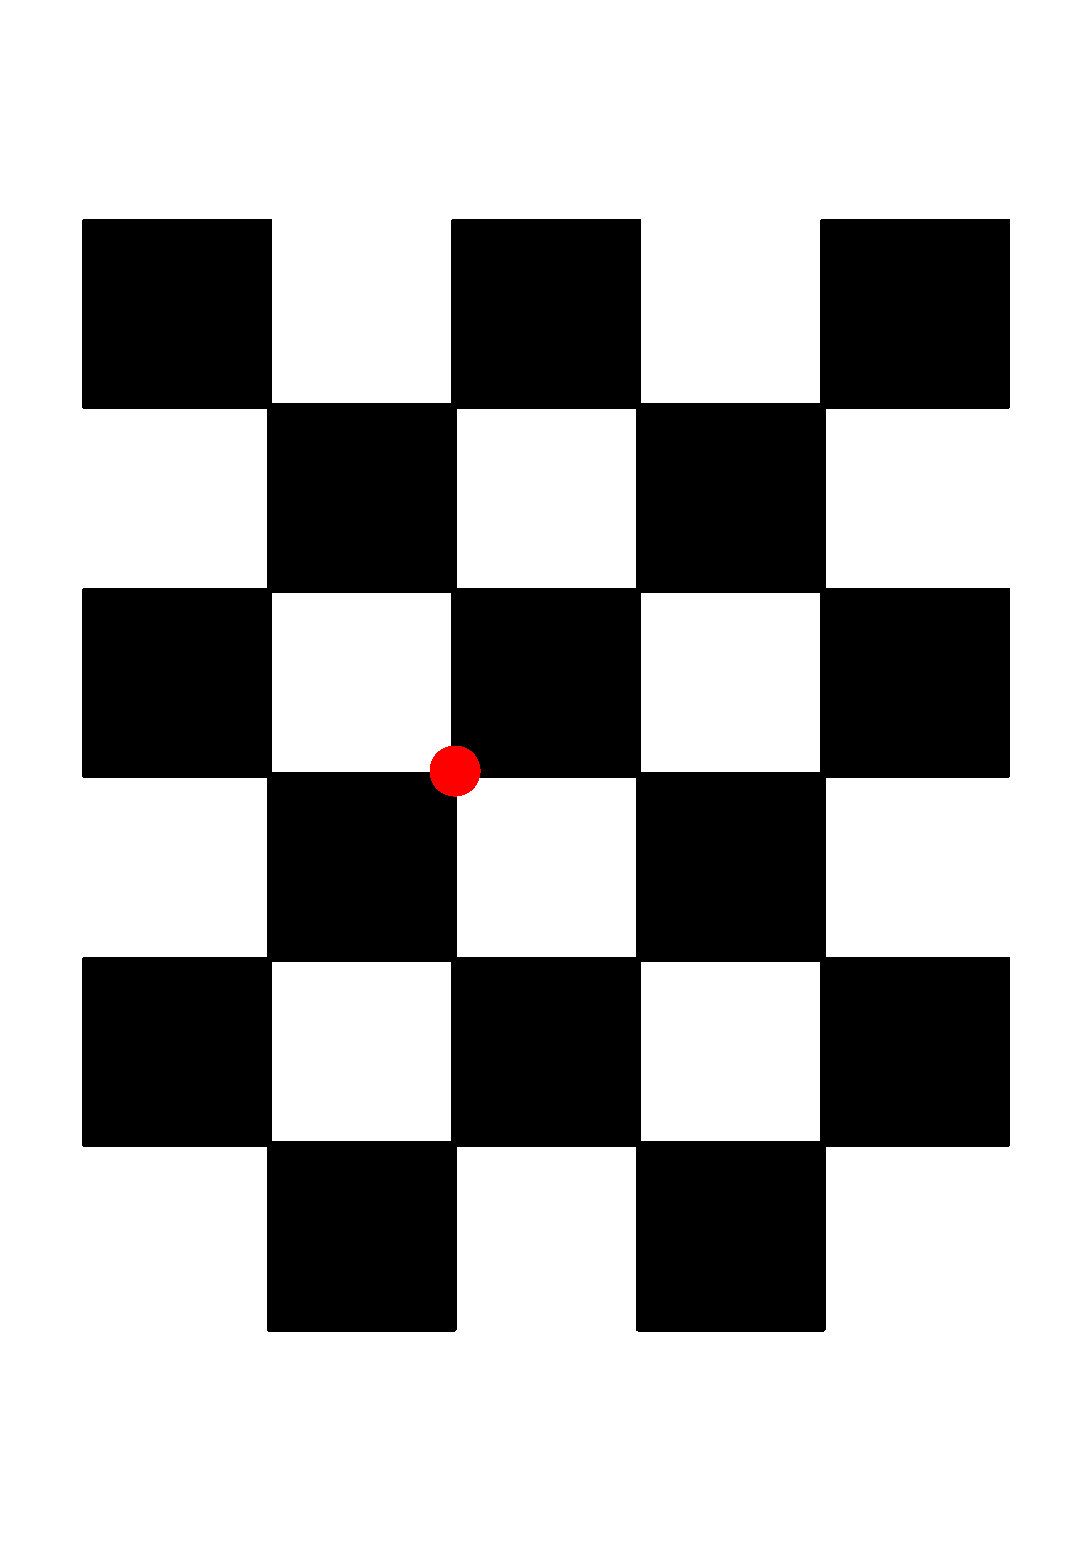
\includegraphics[angle=90, width=0.5\textwidth]{figures/chapter2/chessboard_pattern}
  \caption{An example of a typical chessboard pattern used for calibration.}
\label{fig:chap2-calib-pattern}
\end{figure}

In the case of the chessboard pattern, acquiring the two-dimensional coordinates of the corners is accomplished by using OpenCV's `findChessboardCorners()' and `findCornerSubPix()' functions, which makes use of a Harris corner detection algorithm, first described by~\cite{harris1988combined}, to find the pixel coordinates of the corners on the chessboard pattern. The three-dimensional coordinates is fed to the calibration function according to an axis-system and measurement unit defined by the programmer. These coordinates can be as simple as a vector containing the corner coordinates in square units, e.g.\ the corner from Figure~\ref{fig:chap2-calib-pattern} will then be represented as $(3, 2, 0, 1)$ in homogeneous coordinates (note that $z_w$ will be zero since the board is flat). 

Next, for best calibration results, OpenCV recommends that camera calibration takes place within a well-lit room with a white background, using a calibration pattern with a wide white border in clear view of the camera and at different locations and orientations relative to the camera. These recommendations are mainly to increase the contrast between the black features and the white background and make it easier for OpenCV to accurately find each feature's pixel coordinates. Furthermore, the more diverse the location and orientation data is, the more accurate the estimate for the intrinsic camera parameters will be. 

With the of two-dimensional and three-dimensional data sets recorded, the calibration function can determine the camera matrix $C$. 

\subsection{Principle n-Points Problem}

The Principle n-Points (PnP) problem, as stated by~\cite{horaud1989analytic}, `is the problem of finding the position and orientation of a camera with respect to a scene object from $n$ correspondence points', where the scene object would normally be a well-characterised calibration object or pattern. It is a well-researched sub-field of computer vision with various solutions to the problem that have been proposed. These solutions include the non-iterative solutions, such as the P3P solution proposed by~\cite{gao2003complete} and the PnP solvers by~\cite{lepetit2009epnp} and~\cite{schweighofer2006robust}, and iterative solutions, such as the method proposed by~\cite{lu2000fast}.

It was found that iterative methods produce very accurate results, but can become unstable if its not properly initialised and can take a long time to converge. Conversely, the non-iterative ePnP method by~\citeauthor{lepetit2009epnp} implements~\citeauthor{schweighofer2006robust}'s robust solver and produces results whose accuracy is comparable to those produced by its iterative counterpart. However, it produces these results in a fraction of the time, having a big $\mathcal{O}$ complexity that grows linearly ($\mathcal{O}(n)$), as opposed to competing non-iterative methods which commonly have a big $\mathcal{O}$ complexity to the order of 4 or more ($\mathcal{O}^4(n)$). On the downside, the accuracy of the ePnP's methods results is fairly dependant on the number of sample points, i.e.\ the number of point correspondences between the three-dimensional features and their two-dimensional projections. 

The OpenCV library has implementations of the P3P and ePnP methods, as well as its own implementation based on Levenberg-Marquardt [\cite{levenberg1944method} and~\cite{marquardt1963algorithm}] optimisation, where the pose (i.e.\ the combination of translation and rotation vectors) that minimises the reprojection error, that is the sum of the squared distances between the actual two-dimensional points and the projected two-dimensional points, is determined and selected. 

OpenCV's `solvePnP()' function can be used to determine the pose of a camera relative to a calibration pattern. This can be accomplished as follows. After the camera calibration procedure, the intrinsic parameter matrix $N$ from Equation~\ref{eq:chap2-cam-intrinsic} is determined. Then, using a calibration pattern, a set of three-dimensional object coordinates and its corresponding two-dimensional projection can be obtained. Following from Equation~\ref{eq:chap2-2d-to-3d}, with the matrix $C$ and two-dimensional image projections and three-dimensional object coordinates, the pose matrix $P$ can then be found. This matrix then contains the translation and rotation data for the camera relative to the calibration pattern. 

\subsection{Random Sample Consensus}

SPEEL MET RANSAC WAARDES IN OPENCV OM PUNTE AF TE SKAAAAAAAT

For both the camera calibration and PnP solving functions, two-dimensional image projection data of three-dimensional object data is required. As mentioned, OpenCV's `findChessboardCorners()' function can automatically detect corner features on a chessboard pattern and provide the two-dimensional projection data. However, the methods employed are prone to erroneously classifying some features as corners, introducing unwanted noise into the system. 

To remedy this,~\cite{fischler1981random} proposed a new algorithm to iteratively sift through a data set and reject any outlier data. This algorithm is dubbed Random Sample Consensus (RANSAC) and is a commonly used method in the computer vision field where it is used to determine if an image feature, e.g.\ a corner on a chessboard, that has been classified as such, has been classified correctly. 

\section{Machine Learning Algorithms}

\subsection{Introduction}

\subsection{Radial Basis Function}

\subsection{Artifical Neural Network}

\subsection{Linear Interpolator}
